\documentclass[12pt, oneside]{article}
\usepackage{graphicx} % Required for inserting images
\usepackage{cite}
\usepackage{amsmath,amssymb,amsfonts}
\usepackage{algorithmic}
\usepackage{graphicx}
\usepackage{textcomp}
\usepackage{xcolor}
%\usepackage{hyperref}

\usepackage{IEEEtrantools}


\begin{document}

\begin{titlepage}
    \begin{center}
        \vspace*{1cm}
        {\huges
        \center{\huge{\textbf{Dissertation Research Proposal}}}}
         \\
         \vspace{0.3cm}
         \large{Self-organised Resource Sharing for Decentralised Multi Agent on 2D plane Based on STDMA}
         \vspace{0.5cm}
        \\
        {\large By}
        \\
        \vspace{0.5cm}
        \textbf{Runze Yuan}
   		\vspace{1.5cm}
        \\
        \vspace{0.25cm}
       
\includegraphics[scale=0.6]{logos/bristolcrest_colour.pdf}
        \hspace{5mm}
        
\includegraphics[scale=0.35]{logos/UWE_insignia.png}

        \vspace{10mm}
        {\large Department of Engineering Mathematics\\
        \textsc{University of Bristol}}
        \\
        \&
        \\
        {\large Department of Engineering Design and Mathematics\\
        \textsc{University of the West of England}}\\

        \vspace{0.8cm}
 
        \vspace{0.8cm}
        \today
        
    \end{center}
    
\end{titlepage}

\tableofcontents
\pagebreak


\section{Aims and Objectives}
\subsection{Aims}
Based on the self-organised channel resource allocation principle of the STDMA(Self-organised Time Division Multiple Access) \cite{STDMA} communication protocol, develop a method for agents to achieve collision-free moving on a 2D plane, make it self-organised, decentralised and scalable. 
\subsection{Objectives}
\label{Objectives}
\begin{itemize}
    \item Develop a multi agent communication scenario with STDMA in ROS2. In this scenario, multiple identical agents will share the same channel and all agents have both receiving and transmitting capabilities. The goal is to enable agents to autonomously organise/join the communication process after start up.
    % 使用ROS2与其node实现多agent的通信场景模拟。在此场景中,多个相同的agent将共享同一个信道,且agent都具有收发功能,agents应当能自动地组织/在开机后加入通信过程。目标是使agent能够在开机后自主地组织/加入通信过程。
    \item On the basis above, a simple grid world is implemented: a 2D map composed of grids, each grid representing a part of space. Agents would move from one grid to another on the map.
    % 在上述基础上实现简单的二维地图导航情景:一张由若干网格组成的二维地图,每一个网格代表空间的一部分。agent的运动就是在地图中从一个格子移动到另一个格子。格子的形状不仅限于四边形[],这里需要后续进一步研究确定。
    \item Using the principle of STDMA \cite{STDMA} to implement simple decentralized conflict-free space(which is a kind of resource) sharing and simulate implementation in the above scenario.
    % 用STDMA的原理实现简单的去中心化无冲突空间(其也是某种资源)分享,并在上述场景中模拟实现。
    \item STDMA is designed for 1D resource sharing (slots in time frames), and directly applying STDMA for 2D space sharing will definitely lead to some deadlock and inefficient scenarios\cite{MAPF_Deadlock_Explain1}\cite{MAPF_Deadlock_Explain2}. Determine the cause of this problem by observing the experiment, and make corresponding improvements to this problem. 
    % 直接套用STDMA一定会导致某种死锁和低效的场景发生[]。通过实验模拟定位此类场景发生的原因并进行改进,设计一些资源分享中的规则,并提升算法的表现。
    \item Use appropriate performance metrics (makespan, sum and average of path length, number of conflicts) to evaluate the advantages and disadvantages of algorithm performance. 
    % 选取合适的性能指标,评判算法性能的优劣。
\end{itemize}

\pagebreak

\section{Motivation}
%几个灵魂问题:
% 1. 你的研究重要在哪儿?
% 2. 为什么应用需要此种改变?
% 3. 为什么你的方法能带来这种改变?
% 4. 难在哪儿?
% 5. 创新在哪儿?
% 6. 为什么是你?
\subsection{Why multi agent system in a 2D world?}
% 解释去中心化多智能体系统的应用
% 物流运输,制造业,电力系统,等等。
% 中心化控制方法在大规模应用时往往受到以下限制:计算量的限制,较不灵活,且容易产生single point failure(失去系统中的关键决策者)。为了克服上述缺点,需要研究去中心化控制方法。
% 
%多智能体系统技术由于其灵活性和智能性等出色特点而得到了快速的增长和发展,这些特点在解决复杂的分布式问题时非常有用。 多智能体系统通过其协调、通信和协商等新兴特征,能够处理现实世界问题的复杂性。 多智能体系统也被视为一种技术和工具,有助于分析和开发大规模分布式系统或以人为中心的系统的新模型和理论。

% edge computing 的上升趋势可以作为一项证据
% 
% 得益于设备计算能力的增长和智能设备的普及,智能设备之间协调的话题越来越受到关注。
%The topic of collaboration between intelligent devices is becoming more and more popular thanks to the growth of device computing power and the popularity of intelligent devices. And that leads to the research of multi agent systems.

% 智能可穿戴设备的趋势图here, 多智能体系统的柱状图here

% 多智能体系统所具备的去中心化的灵活性和鲁棒性在面对复杂的分散式问题时非常有效[]。传统的中心化系统的缺陷如:single point failure, 计算量对规模的限制,对于去中心化的multi agent system 来说都不是问题。
%The decentralised flexibility and robustness of multi agent systems are very effective when faced with complex distributed real-world problems\cite{Why_MAS_1}. The drawbacks of traditional centralised systems, such as single point failure and the computational limitation on system size, are significantly reduced in decentralised multi agent systems.

% 关于多机器人集群

% 这个研究题目的设想主要来源于仓库自动化中所使用的AGV机器人[]。AGV机器人的主要用途在于室内地点或仓库环境下的物料搬运,此种机器人在工业4.0和柔性生产需求提升的背景下有较好的发展前景。

The idea for this research topic comes from the usage of Auto Guided Vehicles (AGV) \cite{AGV_explained} in warehouse automation. A typical AGV system is composed of many identical carrier robots and mainly used for unmanned cargo transporting in indoor environments (which could be \textbf{represented by a 2D plane}). Market demand for AGV is rising in the context of Industry 4.0 and the increasing demand for flexible manufacturing\cite{Industry_4.0}.

% 在新的生产需求下,传统的中心化AGV控制方法逐渐不适用于新的使用场景。中心化的控制方法由于其对内存,通信,计算的限制,将其应用于更大规模的系统是很困难的。生产制造逐渐向去中心化提出要求[]。本研究的主题就是要实现一定程度的去中心化控制,

In new production requirements, traditional centralised AGV control methods are gradually unsuitable for new application scenario. Centralised control methods are difficult to apply to larger systems due to their limitations on memory, communication, and computation. Production manufacturing is gradually demanding decentralised control\cite{Industry4.0_decentralised}.

% 本研究主题中要解决的主要是AGV的路径空间分享问题。对于这一问题,一般将其视为某种multi agent system分类下的资源分享/路径规划问题。

    The main focus in this research topic is the space sharing problem of AGV. For this problem, it is generally regarded as a resource sharing/path planning problem in multi agent system domain\cite{AGV_Review_2020}. Take AGV robots as agents, and all the agents should \textbf{resolve the resource (limited space in operating environment) sharing problem without a centralised controller.}

\begin{figure}
    \centering
    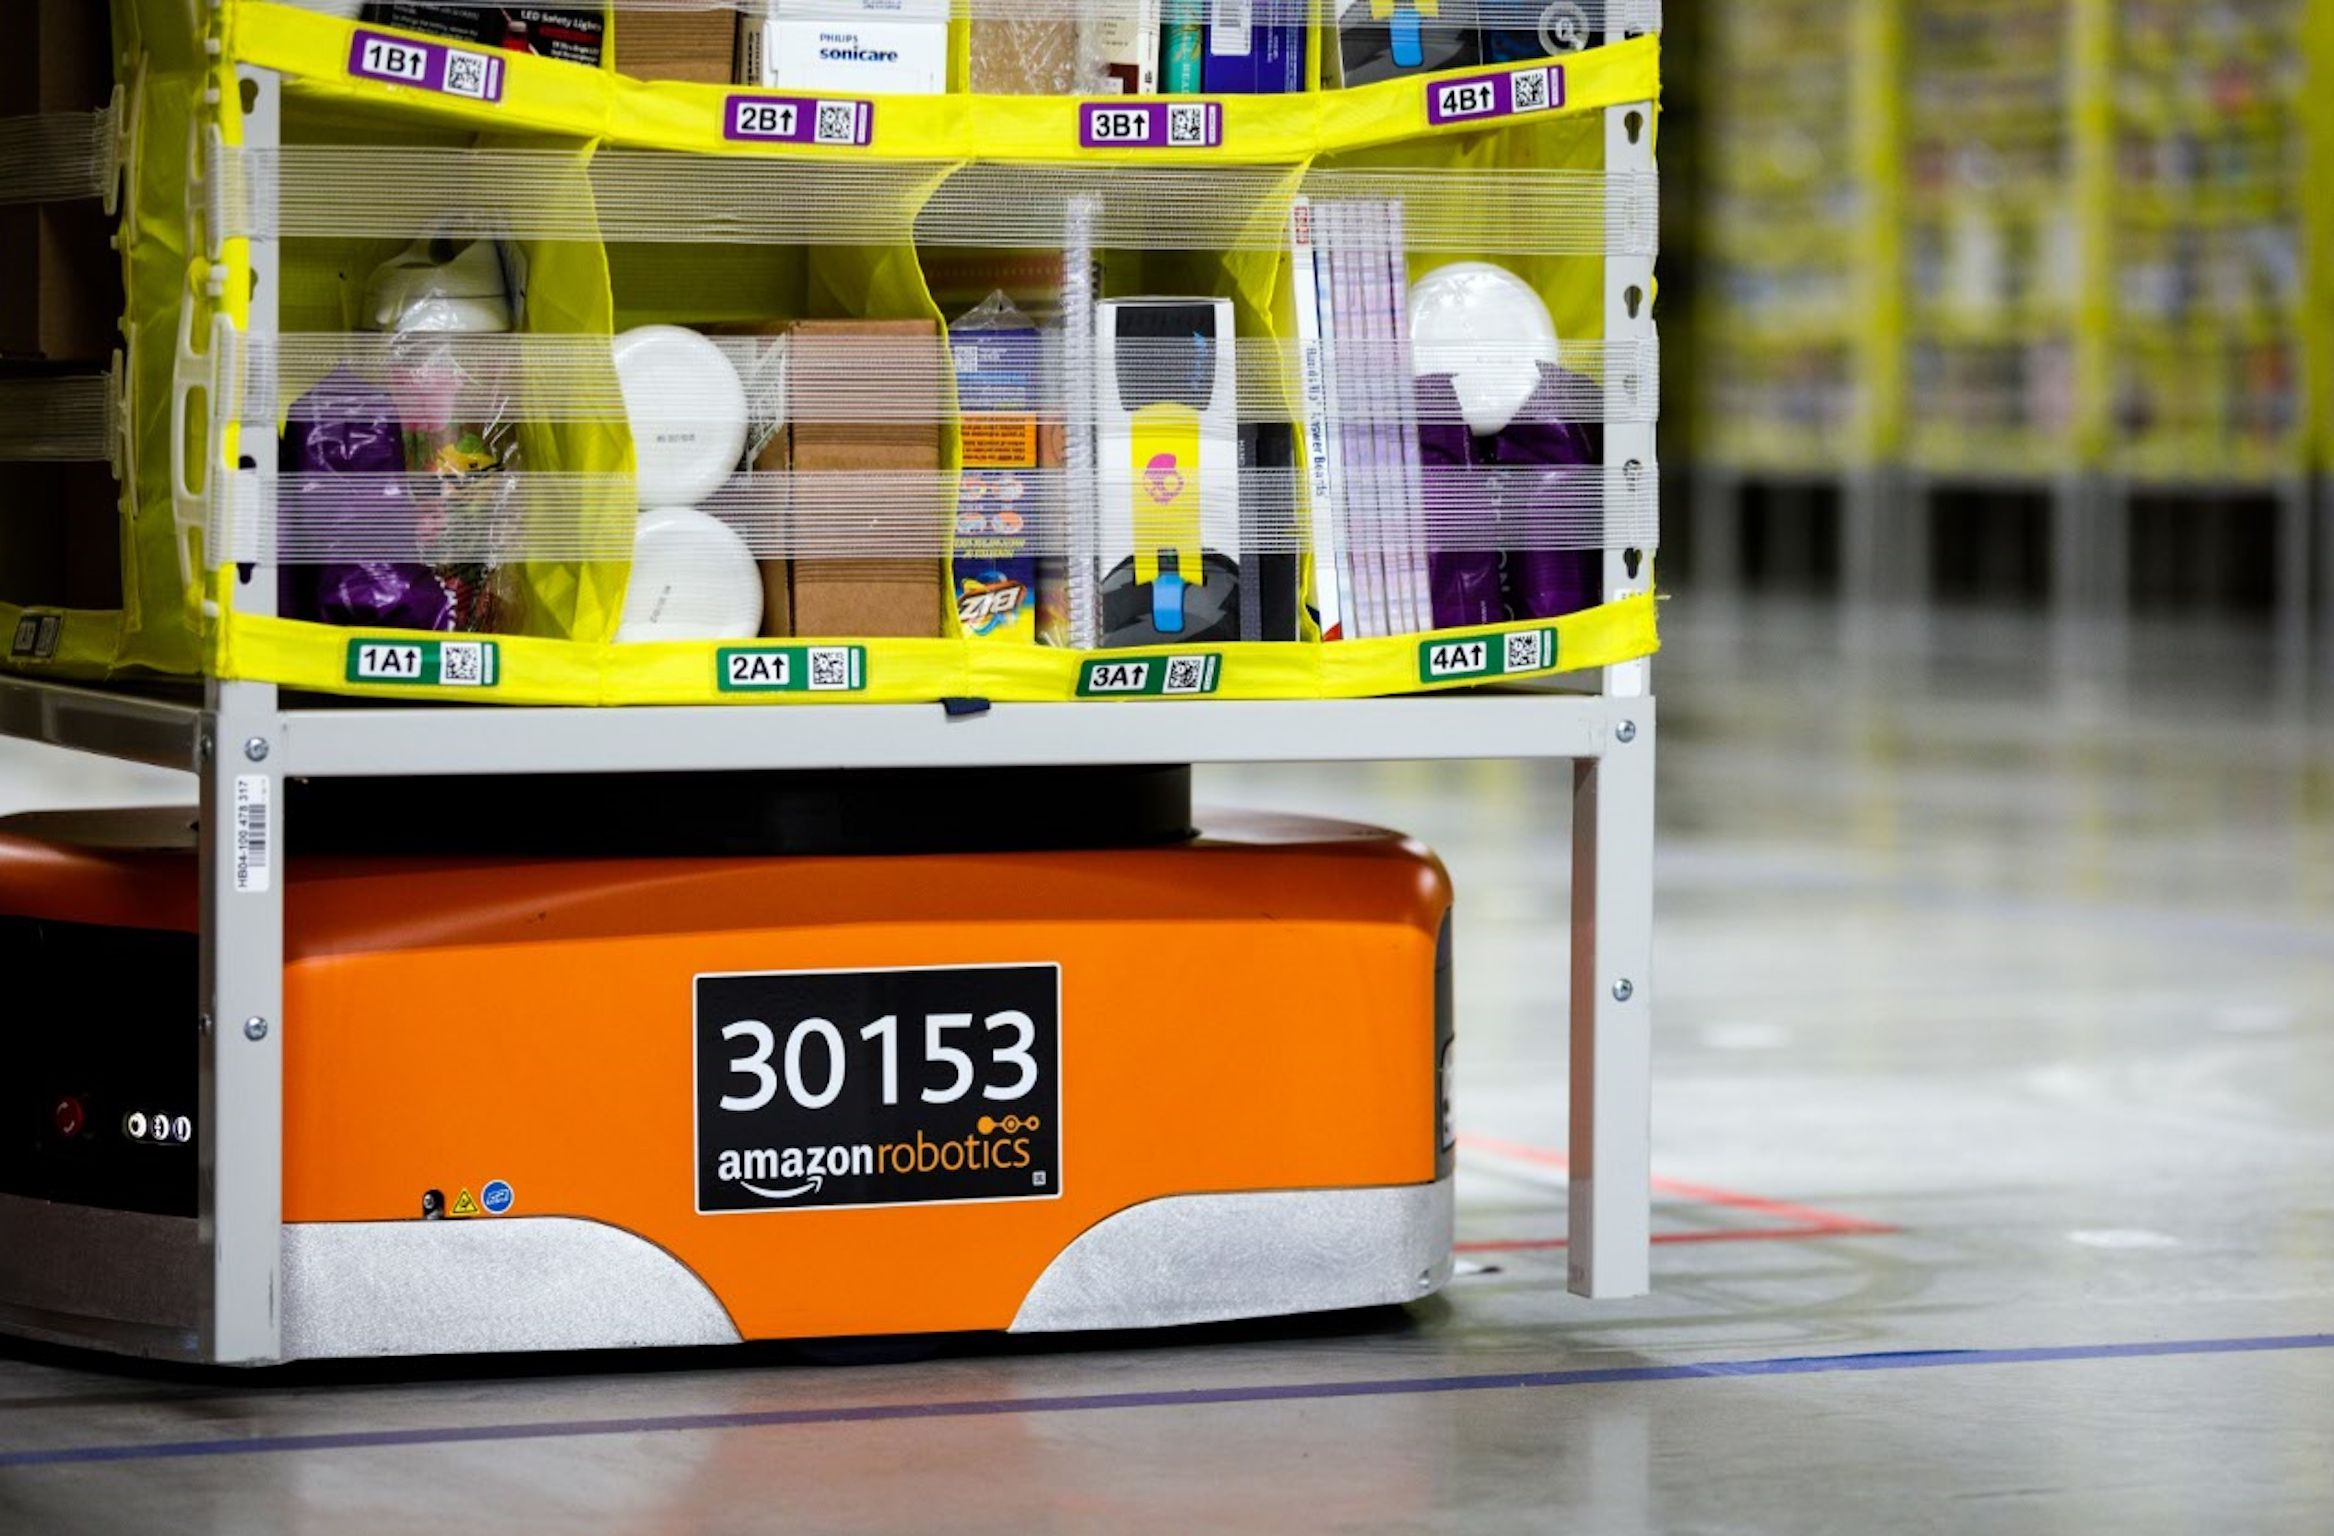
\includegraphics[width=0.6\linewidth]{figs/Amazon_Warehouse.jpeg}
    \caption{Example of AGV: Kiva system operating in Amazon warehouse.\footnotemark }
    \label{fig:Amazon Warehouse Robots}
\end{figure}

\footnotetext{https://spectrum.ieee.org/interview-brad-porter-vp-of-robotics-at-amazon}

\subsection{Why STDMA?}

Self-organised Time Divided Multi Access (STDMA) is a field-tested \cite{STDMA_field_usage} channel access method which based on a set of policies about how  should the agents apply for slots in repeating frames (details explained in Section \ref{Literature_Review}). 

% 选用STDMA的原因:现有的此领域研究有很严重的research gap:大多数研究假设通信不受限制,并对通信条件有苛刻的要求[],并只专注于资源的共享方案。
Reasons for using STDMA: Existing research has huge research gap in this field. Most studies assume that communication between robots is ideal \cite{Current_Research_Gap} and only focus on resource sharing schemes, which leads to strict communication requirements that are not practical.

% 利用STDMA的原则构建机器人之间的通讯【cite 第一段】可以将去中心化自组织特性带入通讯条件的构筑中,缩小这一gap。但是时分复用通讯也有其局限性,因为通讯将会是串行的,所以资源分配方案的设计会受到一些影响。由于此串行的
Using STDMA to build communication between robots (like previous mentioned in Section \ref{Objectives}) can bring decentralized self-organising characteristics into the formation of communication process, narrowing the research gap. 

However, using STDMA for communication also has its limitations, because communication between robots would be serial, and robots must take turns to speak. In such condition the design of resource sharing schemes will be affected for robots have to wait for their turn to send messages. Using principles from STDMA again  to build the resource sharing scheme after we have self-organised communication based on STDMA seems feasible and make sense, because the limitation in communication is inherited from the STDMA protocol, and STDMA is complete on its own. But there could be other potentially better solutions, and without simulations I cannot answer this question yet. 

The most challenging part could be developing appropriate resource sharing scheme in STDMA based communication environment.

% 这里还需要大改,把challenge提出来,然后还要更贴合他提出的几个问题 记得参考他给的pdf改。那样灵感会多很多
% 提出STDMA的优势:简单并只关注于可用的格子。

% 许多
\pagebreak

\section{Literature Review}
\label{Literature_Review}

% literature review 应当总结出一个结构,并在开始写之前心里有个数

% 我的literature review:

% 此研究主题面临的主要问题是:使多智能体自组织通讯并实现无碰撞的移动。
The challenges in this research topic is to enable self-organised communication with STDMA and collision-free movement of multi agents.
\subsection{Self-organised communication with STDMA}
% STDMA是一种MAC技术,主要用于无线网络的自组织通讯。其已被用于AIS(13年的那个的7)和VDL(13年那个的4),也有研究评估过STDMA在工厂环境中的应用以及用于车对车通讯的表现。其应用前景是可观的。接下来是STDMA原则的简单介绍。
% 作为一种TDMA协议,STDMA将时间划分为等长度的帧,并将帧划分为若干个大小相等的槽。STDMA的基础假设是,所有的站点都有同步的时钟。工作站点的生命周期有四个阶段:初始化,网络进入,第一帧与连续运行。
% 1. 初始化:站点监听一个完整的帧,确定帧中槽位的使用状态。后续将根据使用状态信息进行槽位的保留和申请。
% 2. 网络进入:从可用的槽位中根据RTDMA的P持久【】选择一个,用此槽位宣布自身的存在,同时再为自己保留一个槽位。
% 3. 第一帧: 在网络进入阶段中所保留的槽位里,进一步为自己保留更多槽位以满足工作需求(一定大小数据包的的传输)。每个槽位都有随机的超时时间,达到超时时间后槽位将被释放
% 4. 连续运行:正常使用第一帧阶段保留的槽,若有槽过期则再次进行槽位的保留。

% STDMA协议的性能主要受限于以下两个方面:
% 冲突:多个站点选择了同一个槽。
% 可用槽位不足:当可用插槽数量不足时,站点将被迫与与其最远的站点共用插槽。

% 对于上述问题,有一些文章从插槽选择策略和算法参数方面提出了改进[老师的那个],[刚找的那个]。

STDMA\cite{STDMA} is a technology primarily used for self-organising communication in wireless networks. It has been used in AIS and VDL mode 4\cite{STDMA}, and there are also several studies evaluating its potential as a protocol for industrial applications\cite{STDMA_for_industry}.

As a TDMA protocol, STDMA divides time into frames of equal length and divides the frames into a number of equally sized slots. the assumption of STDMA is that all sites have synchronised clocks. The life cycle of a working site has four phases: initialisation, network entry, first frame and continuous operation.

Initialisation: Site listen to the channel for an entire frame, and determine the current allocation of slots. Subsequent phases would use unallocated slots to operate.

Network Entry: Use an unallocated slot to announce its existence, and reserve one more slot for the next phase.

First Frame: Use the slot reserved in the previous phase to reserve more slots to meet the work requirements. Each slot is assigned with a random time duration and will be released once exceeded. 

Continuous Operation: Use slots reserved in the first frame phase to operate, and reserve slots again once they are released.

The main constraints for STDMA are:
(1) Collision: Multiple sites accidentally used the same slot, most likely to happen in network entry phase for sites has not yet announced its existence. (2) No available slots: More slots needed than exist, and sites are forced to use slots assigned to other sites. 

For its constraints, there are several improvements for the slot arranging strategies \cite{STDMA_rule_improv1} and duration of slots and frames \cite{STDMA_para_improv1} \cite{STDMA_para_improv2}. But this is not the focus of this research.



\subsection{Collision-free movement}

% 一般来说,多智能体在空间中无碰撞移动的问题是某种任务分配/路径规划问题。此种问题将智能体在空间中的移动抽象为某在无向图中的移动,图中的节点代表空间,边代表空间之间的连接。这里的关键约束在于,智能体使用的路径之间应当没有碰撞,也就是

In general, the problem of collision-free movement of multiple agents in space is taken as a part of \textit{Multi Agent Path Finding} (MAPF) \cite{MAPF_Deadlock_Explain1} problem, and MAPF has several subtypes like \textit{Multi Agent Pickup and Delivery}(MAPD), \textit{Multi Agent Multi Item Pickup and Delivery}(MAMPD)\cite{MAMPD}. Research in these subtypes are for the scenario of \textit{lifelong} MAPF: Agents in the system are in a constant task stream of picking up and delivering, which bring the problem beyond the one-shot solution. Due to the high degree of overlap between domains and potential naming confusion, these subtypes will not be presented separately below.

The scenario defined in Section \ref{Objectives} is like classical MAPF definition. For a system consisting of $n$ agents, the MAPF problem consists of the following three inputs. 
\begin{enumerate}
    \item \textbf{Environment}. Environment is assumed to be priori known and described as an undirected graph $G = (V,E)$, whose vertices $V$ represent space in the environment and edges $E$ describe the connection of vertices.
    \item \textbf{Source}. Starting vertices of the agents. Represented with $s:[1,...,n]\rightarrow V_{s}$, which maps $n$ agents to the source vertices $V_{s}$.
    \item \textbf{Target}. Goal vertices of the agents. Represented with $t:[1,...,n]\rightarrow V_{t}$, which maps $n$ agents to the target vertices $V_{t}$.
\end{enumerate}

Time is assumed to be discrete steps. In each step, agents can only take one action $a(v)=v'$ which is a function that maps the current vertex $v$ to the next vertex $v'$. Agents have two potential actions: \textit{move} and \textit{wait}. \textit{Wait} means the agent will be waiting in the current vertex ($a(v)=v$), and \textit{move} means the agent will move to another neighbouring vertex in graph $G$ ($a(v)=v', (v,v')\in G$). 


% 单智能体计划就是指一系列行动,执行此行动序列可以使智能体从出发点到达目标点。MAPF问题的解就是一个由系统中所有智能体的单智能体计划组成的集合。
A \textbf{single-agent plan} refers to a series of actions $\pi_{n} = (a_{1},...,a_{k})$ that can be executed to move an agent from a source vertex to a target vertex. The \textbf{solution} to the MAPF problem is a set of single-agent plans $\pi=(\pi_{1},...,\pi_{n})$ for all $n$ agents in the system. 

However, there could be conflicts in the solution, which results in collision between agents. Conflicts are defined as different agents are planned to occupy the same edge or vertex in the same time step. \textbf{The aim of MAPF algorithm designing is to minimize conflicts in the solution.}

https://www.mdpi.com/2075-1702/10/9/773






% 根据解决方案的特性可以有以下几种对立的坐标轴:

\section{Impact Assessment}
\section{Risk Register}
\section{Timeline}


\section{References}

\bibliographystyle{plain}

\bibliography{ref}

\end{document}
